%% This is file `elsarticle-template-1-num.tex',
%%
%% Copyright 2009 Elsevier Ltd
%%
%% This file is part of the 'Elsarticle Bundle'.
%% ---------------------------------------------
%%
%% It may be distributed under the conditions of the LaTeX Project Public
%% License, either version 1.2 of this license or (at your option) any
%% later version.  The latest version of this license is in
%%    http://www.latex-project.org/lppl.txt
%% and version 1.2 or later is part of all distributions of LaTeX
%% version 1999/12/01 or later.
%%
%% Template article for Elsevier's document class `elsarticle'
%% with numbered style bibliographic references
%%
%% $Id: elsarticle-template-1-num.tex 149 2009-10-08 05:01:15Z rishi $
%% $URL: http://lenova.river-valley.com/svn/elsbst/trunk/elsarticle-template-1-num.tex $
%%
\documentclass[preprint,12pt]{elsarticle}

%% Use the option review to obtain double line spacing
%% \documentclass[preprint,review,12pt]{elsarticle}

%% Use the options 1p,twocolumn; 3p; 3p,twocolumn; 5p; or 5p,twocolumn
%% for a journal layout:
%% \documentclass[final,1p,times]{elsarticle}
%% \documentclass[final,1p,times,twocolumn]{elsarticle}
%% \documentclass[final,3p,times]{elsarticle}
%% \documentclass[final,3p,times,twocolumn]{elsarticle}
%% \documentclass[final,5p,times]{elsarticle}
%% \documentclass[final,5p,times,twocolumn]{elsarticle}

%% The graphicx package provides the includegraphics command.
\usepackage{graphicx}
%% The amssymb package provides various useful mathematical symbols
\usepackage{amssymb}
%% The amsthm package provides extended theorem environments
%% \usepackage{amsthm}

%% The lineno packages adds line numbers. Start line numbering with
%% \begin{linenumbers}, end it with \end{linenumbers}. Or switch it on
%% for the whole article with \linenumbers after \end{frontmatter}.
\usepackage{lineno}

%% natbib.sty is loaded by default. However, natbib options can be
%% provided with \biboptions{...} command. Following options are
%% valid:

%%   round  -  round parentheses are used (default)
%%   square -  square brackets are used   [option]
%%   curly  -  curly braces are used      {option}
%%   angle  -  angle brackets are used    <option>
%%   semicolon  -  multiple citations separated by semi-colon
%%   colon  - same as semicolon, an earlier confusion
%%   comma  -  separated by comma
%%   numbers-  selects numerical citations
%%   super  -  numerical citations as superscripts
%%   sort   -  sorts multiple citations according to order in ref. list
%%   sort&compress   -  like sort, but also compresses numerical citations
%%   compress - compresses without sorting
%%
%% \biboptions{comma,round}

% \biboptions{}

\journal{Journal Name}

\begin{document}

\begin{frontmatter}

%% Title, authors and addresses

\title{Scheduling Divisible Workloads from Multiple Sources in Network-on-chip Plan}

%% use the tnoteref command within \title for footnotes;
%% use the tnotetext command for the associated footnote;
%% use the fnref command within \author or \address for footnotes;
%% use the fntext command for the associated footnote;
%% use the corref command within \author for corresponding author footnotes;
%% use the cortext command for the associated footnote;
%% use the ead command for the email address,
%% and the form \ead[url] for the home page:
%%
%% \title{Title\tnoteref{label1}}
%% \tnotetext[label1]{}
%% \author{Name\corref{cor1}\fnref{label2}}
%% \ead{email address}
%% \ead[url]{home page}
%% \fntext[label2]{}
%% \cortext[cor1]{}
%% \address{Address\fnref{label3}}
%% \fntext[label3]{}


%% use optional labels to link authors explicitly to addresses:
%% \author[label1,label2]{<author name>}
%% \address[label1]{<address>}
%% \address[label2]{<address>}

\author{Junwei Zhang}

\address{Stony Brook, New York}

\begin{abstract}
%% Text of abstract
This paper is about multiple sources workloads scheduling in Network-on-chip.
\end{abstract}

\begin{keyword}
Divisible Load Theory \sep Processor equivalence \sep Voronoi Diagram \sep Optimal Mass Transport \sep Network-on-chip \sep Monte Carlo Method
\sep Manhattan Distance 
%% keywords here, in the form: keyword \sep keyword

%% MSC codes here, in the form: \MSC code \sep code
%% or \MSC[2008] code \sep code (2000 is the default)

\end{keyword}

\end{frontmatter}

%%
%% Start line numbering here if you want
%%
%%\linenumbers

%% main text
\section{Introduction}
\label{S:1}
Processor Equivalence\cite{robertazzi1993processor} \cite{jia2010scheduling}

There are some properties about the NOC.

\begin{itemize}
\item Each unit core has 4 ports.
\item Each unit core's computation ability and communication ability is the same.
\end{itemize}
There has some variable situation need to be considered.
\begin{enumerate}
\item Each unit core has front-end or not.
\item The number of sources.
\item The source position,for example, corner,edge or inner grid position.
\item The load fraction of each sources. They are even or not.
\item Computation and Communication schema
	\begin{itemize}
	\item Simultaneously computing after receiving the first bit.
    \item Computing after receiving the whole fraction.
	\end{itemize}
\end{enumerate}






\section{Processor Equivalence}

\subsection{Load From Corner}
\begin{itemize}
\item 2*2 regular mesh \ref{unitmesh}
\item 2*3 regular mesh \ref{unitmesh2}
\item 2*n regular mesh \ref{unitmesh3}
\item m*n regular mesh \ref{unitmesh4}
\item Sensitivity Analysis \ref{unitmesh5} \ref{unitmesh6}
\end{itemize}


\begin{figure}[h]
\centering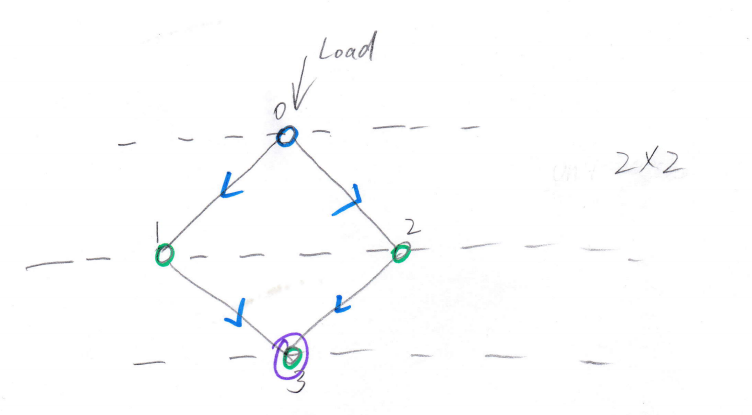
\includegraphics[width=1\linewidth]{unitmesh}
\caption{2*2 regular mesh}
\label{unitmesh}
\end{figure}


\begin{figure}[h]
\centering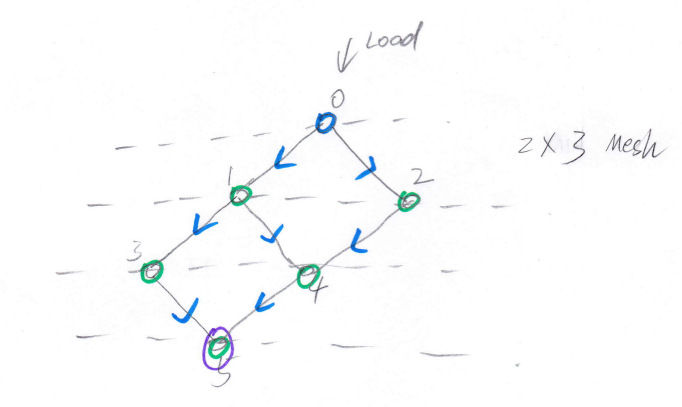
\includegraphics[width=1\linewidth]{unitmesh2}
\caption{2*3 regular mesh}
\label{unitmesh2}
\end{figure}

\begin{figure}[h]
\centering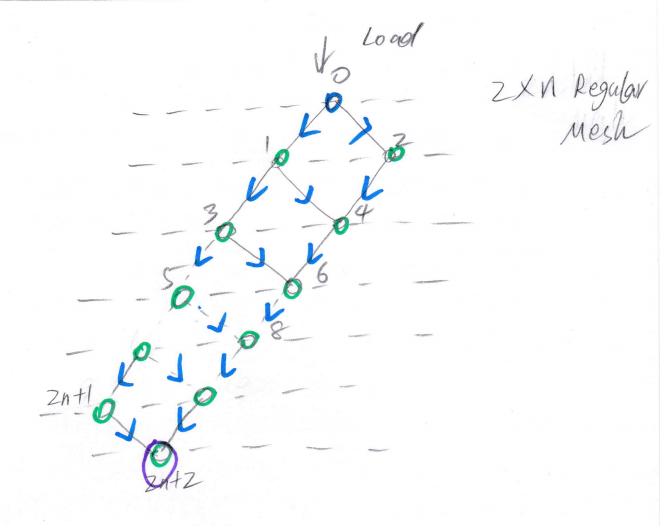
\includegraphics[width=1\linewidth]{unitmesh3}
\caption{2*n regular mesh}
\label{unitmesh3}
\end{figure}


\begin{figure}[h]
\centering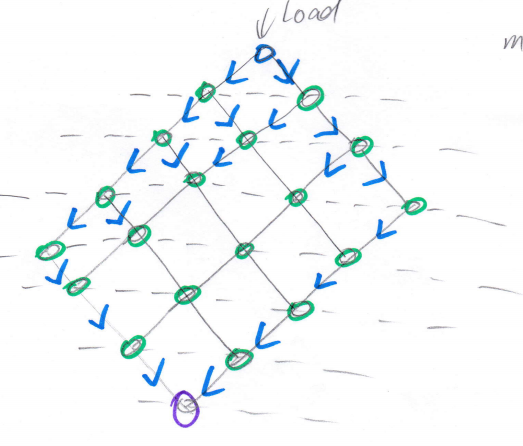
\includegraphics[width=1\linewidth]{unitmesh4}
\caption{m*n regular mesh}
\label{unitmesh4}
\end{figure}



\begin{figure}[h]
\centering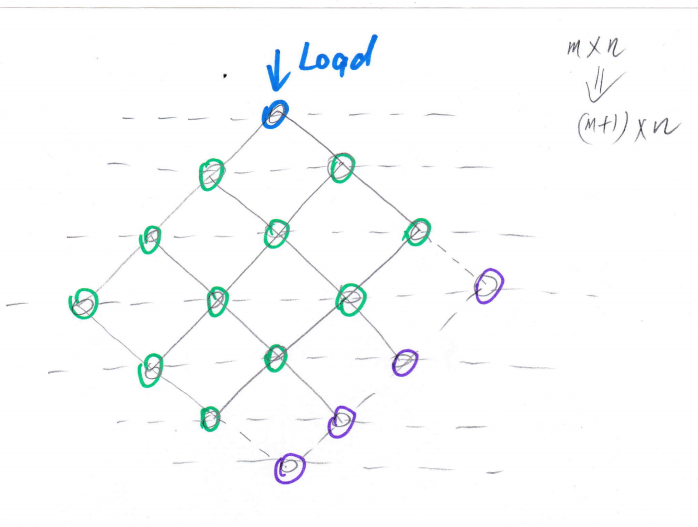
\includegraphics[width=1\linewidth]{unitmesh5}
\caption{Add one column }
\label{unitmesh5}
\end{figure}

\begin{figure}[h]
\centering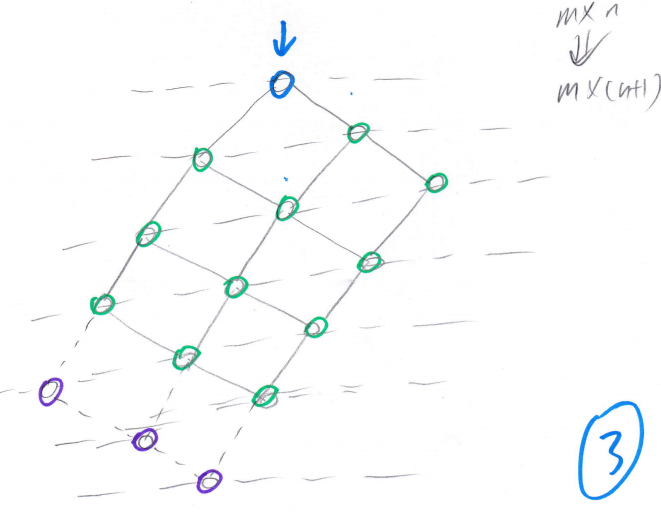
\includegraphics[width=1\linewidth]{unitmesh6}
\caption{Add one row }
\label{unitmesh6}
\end{figure}




\subsection{Processor Equivalence Formula}


\begin{itemize}
	\item Simultaneously computing after receiving the first bit.\ref{eq1}
    \item Computing after receiving the whole fraction.\ref{eq2}
\end{itemize}

\begin{figure}[h]
\centering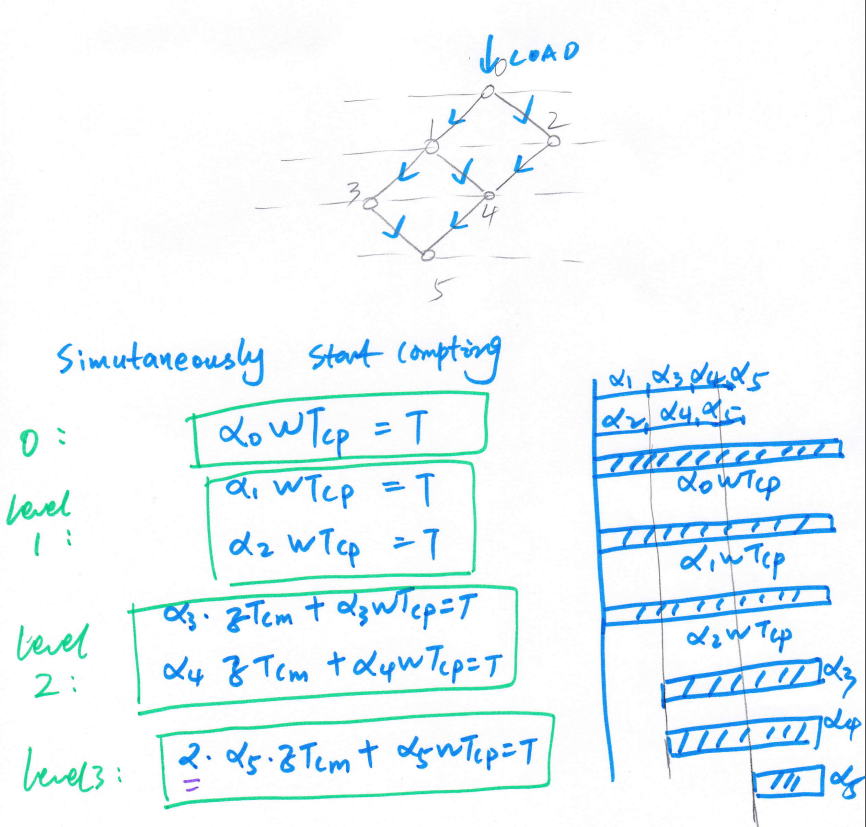
\includegraphics[width=1\linewidth]{eq1}
\caption{Simultaneously computing after receiving the first bit }
\label{eq1}
\end{figure}



\begin{figure}[h]
\centering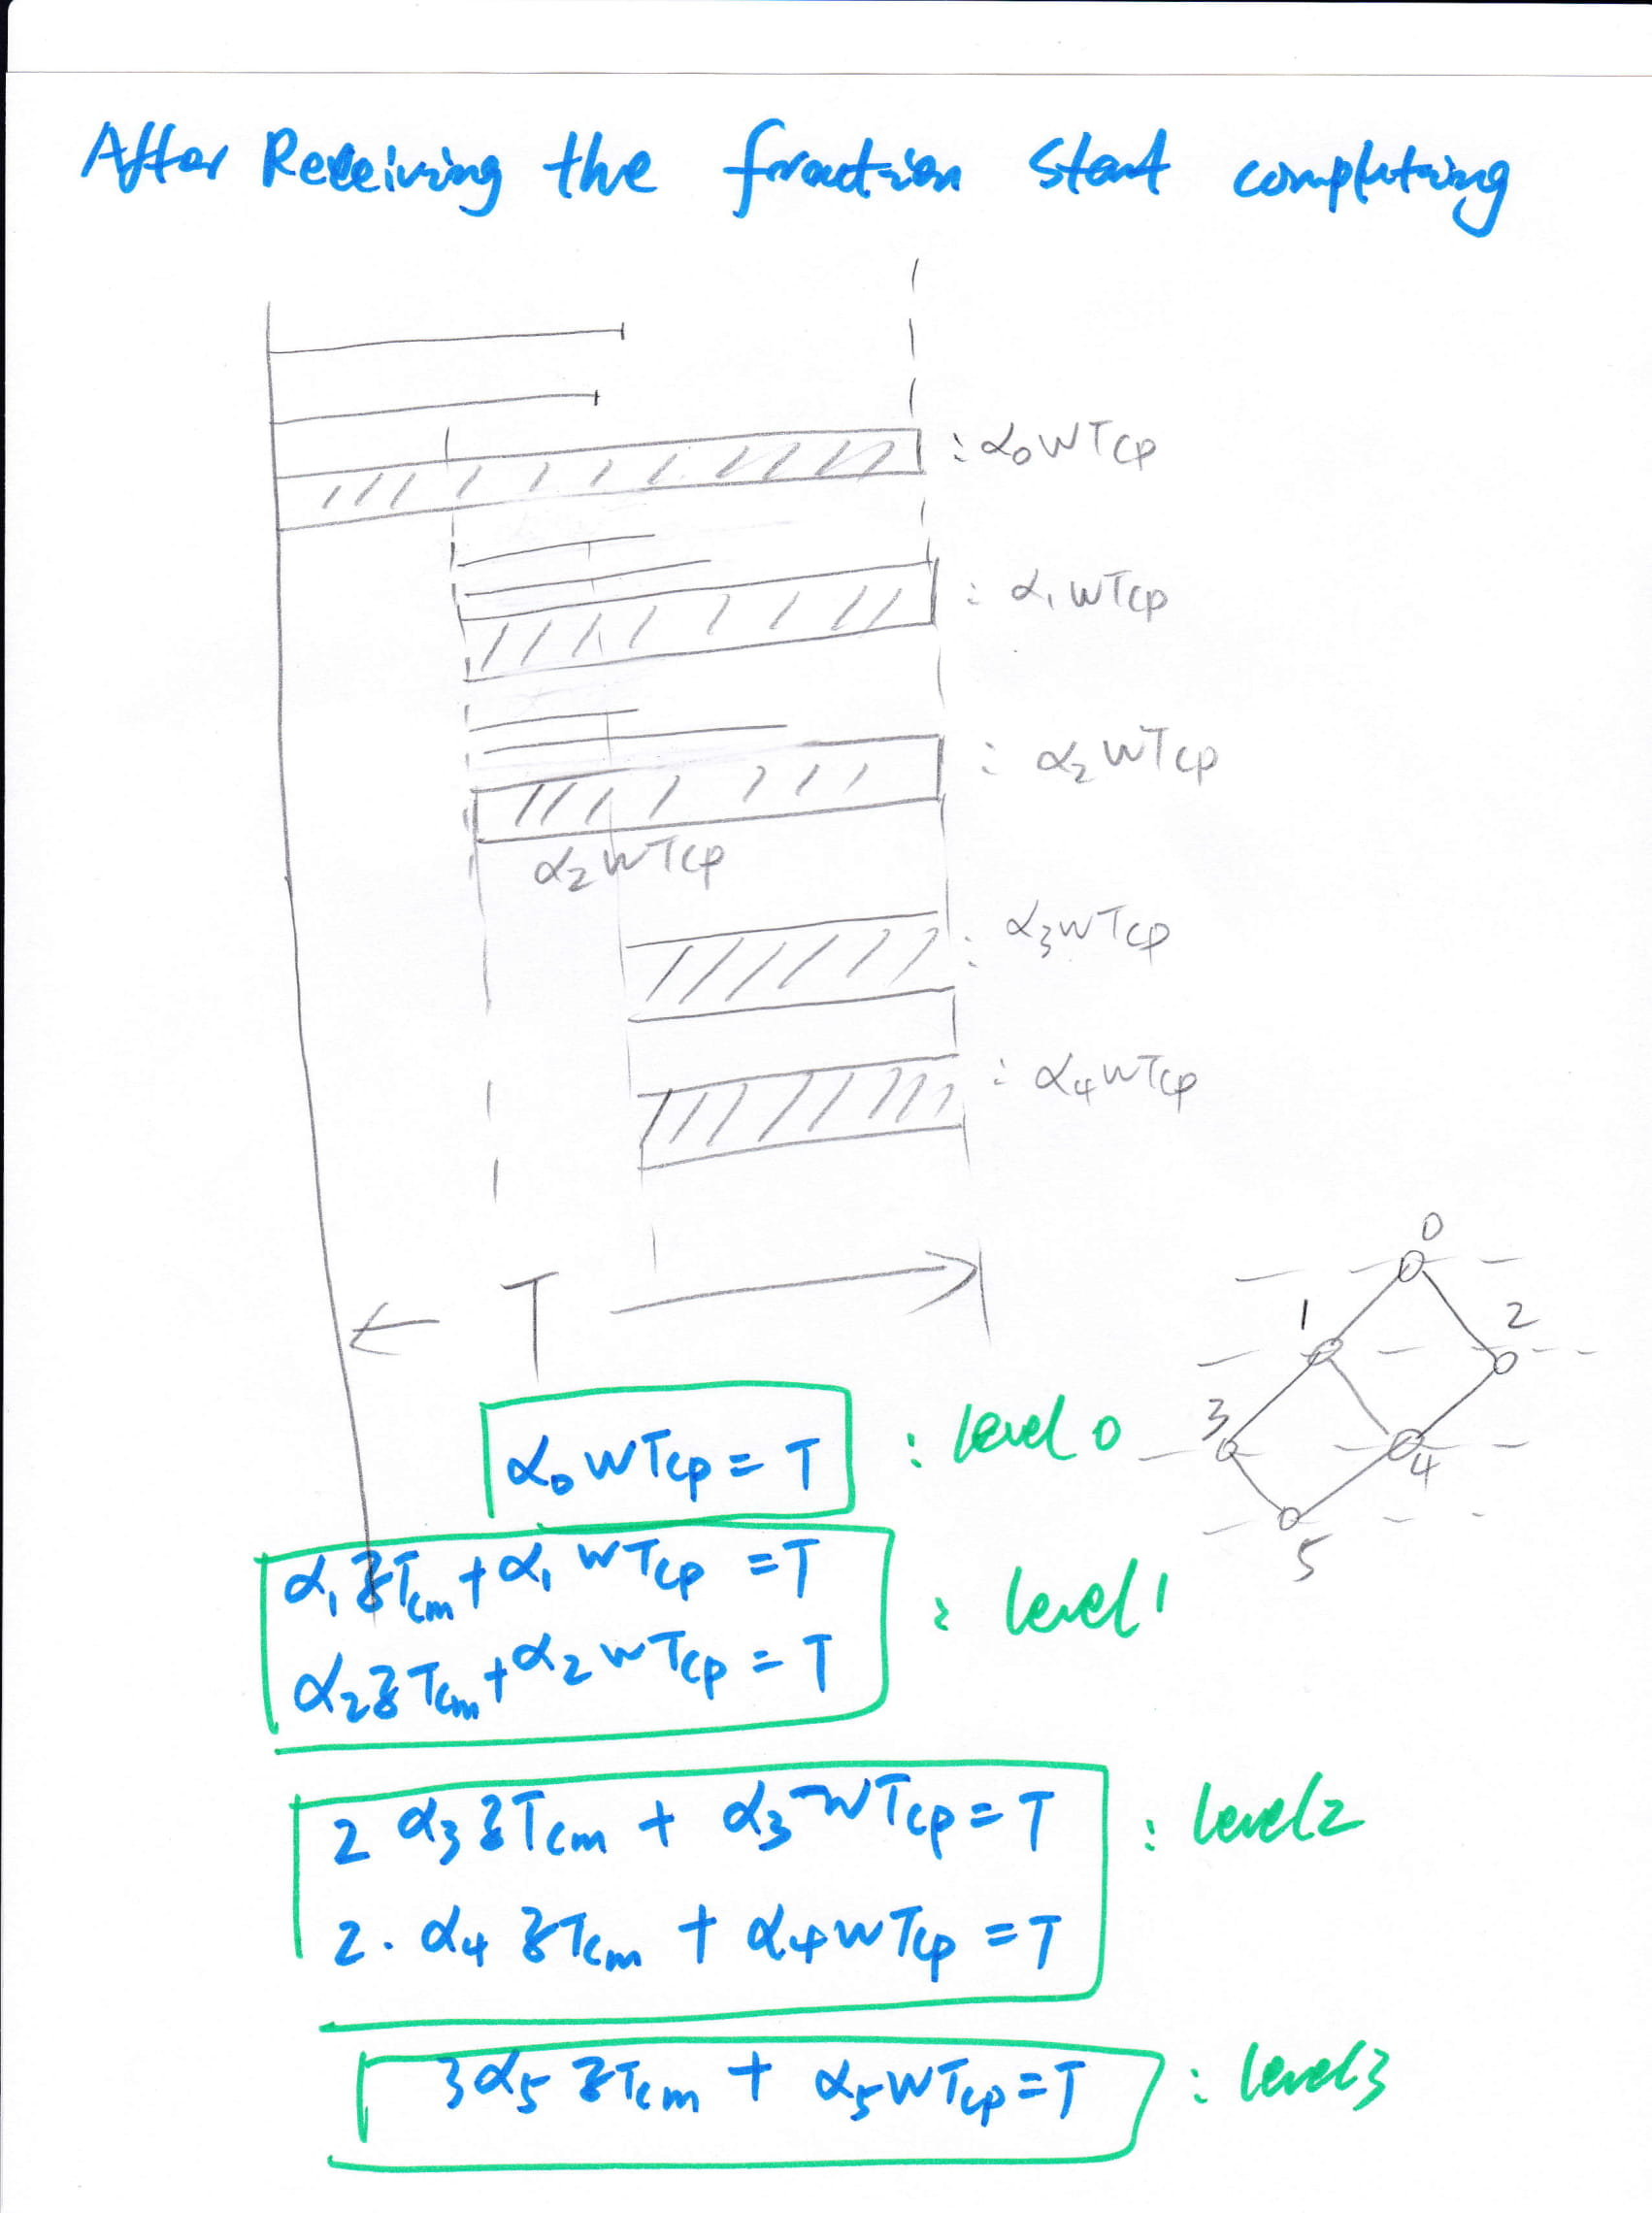
\includegraphics[width=1\linewidth]{eq2}
\caption{Computing after receiving the whole fraction}
\label{eq2}
\end{figure}



\subsection{Load From Edge}

\begin{itemize}
\item Load from edge grid point. \ref{edge1}
\end{itemize}

\begin{figure}[h]
\centering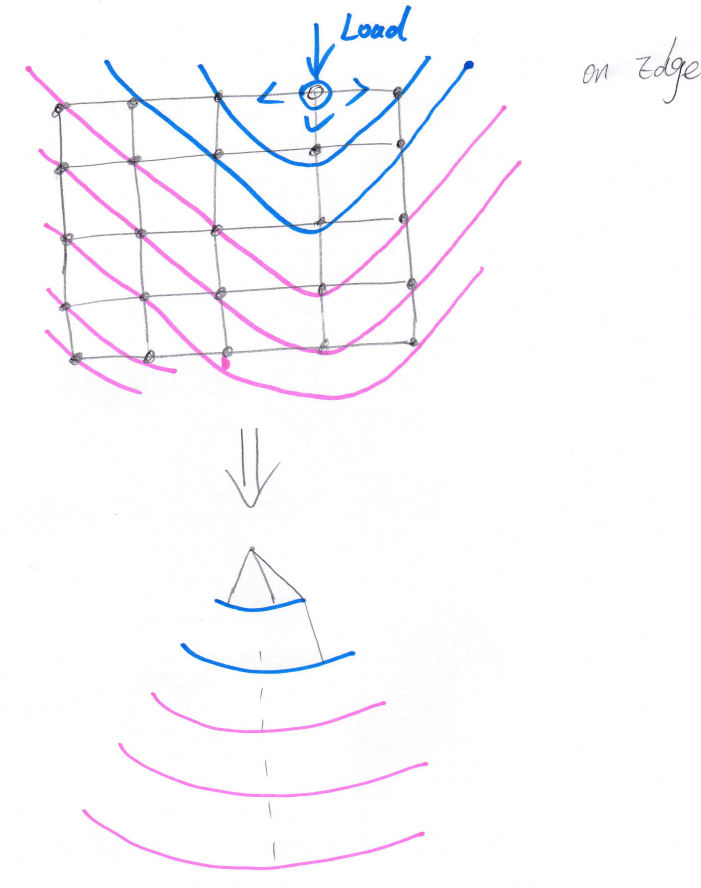
\includegraphics[width=1\linewidth]{edge1}
\caption{Load from edge grid and the contour line }
\label{edge1}
\end{figure}



\subsection{Load From Inner Grid Point}
\begin{itemize}
\item Load from inner grid position. \ref{edge1}
\end{itemize}

\begin{figure}[h]
\centering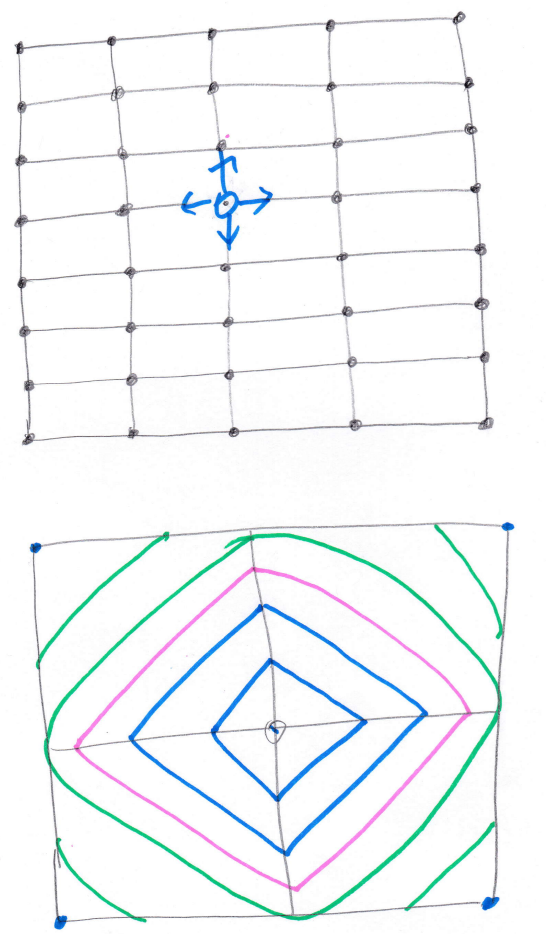
\includegraphics[width=0.8\linewidth]{inner}
\caption{Load from inner grid and it's contour line }
\label{inner1}
\end{figure}



\section{Calculate the source subgraph}

\begin{itemize}
\item the sources consist of a whole larger source node.\ref{subgrah1}

\item the load fraction are even.We can calculate the Manhattan Voronoi diagram \ref{voronoimanhattan} directly under the definition of Manhattan distance.\ref{voronoi1}

\item the source load fraction are not even. \ref{voronoi2}
\begin{itemize}
\item Calculate the Manhattan Voronoi Diagram.
\item Calculate the processor equivalence ability.
\item If the ability of each subgraph equals to the corresponding load fraction, then stop.
\item Otherwise, merge the furthest level leaves to other source node voronoi area.(I can explain with you on Tuesday discussion.) \ref{voronoi2}
\end{itemize}
\end{itemize}


\begin{figure}[h]
\centering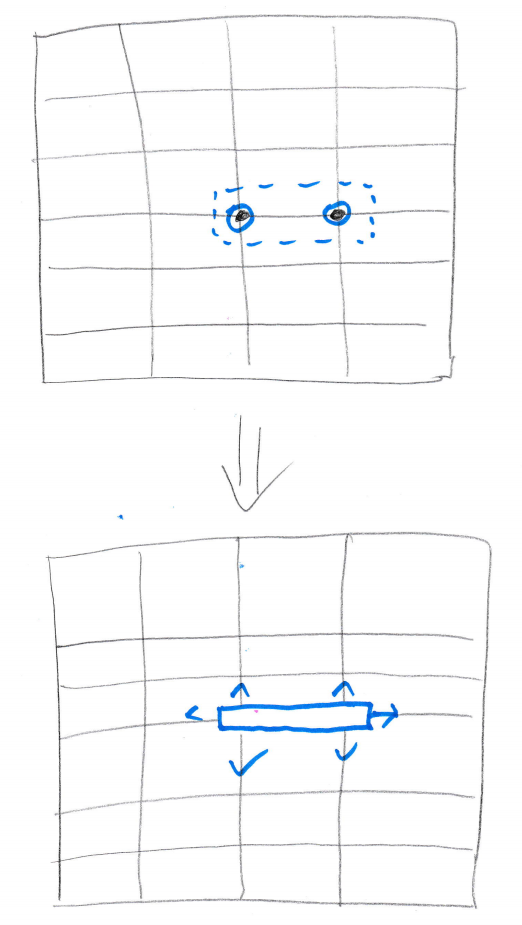
\includegraphics[width=0.7\linewidth]{subgraph1}
\caption{Two source node consists of a whole source node. }
\label{subgrah1}
\end{figure}


\begin{figure}[h]
\centering
\includegraphics[width=0.7\linewidth]{voronoi-manhattan}
\caption{Two source node consists of a whole source node. }
\label{voronoimanhattan}
\end{figure}


\begin{figure}[h]
\centering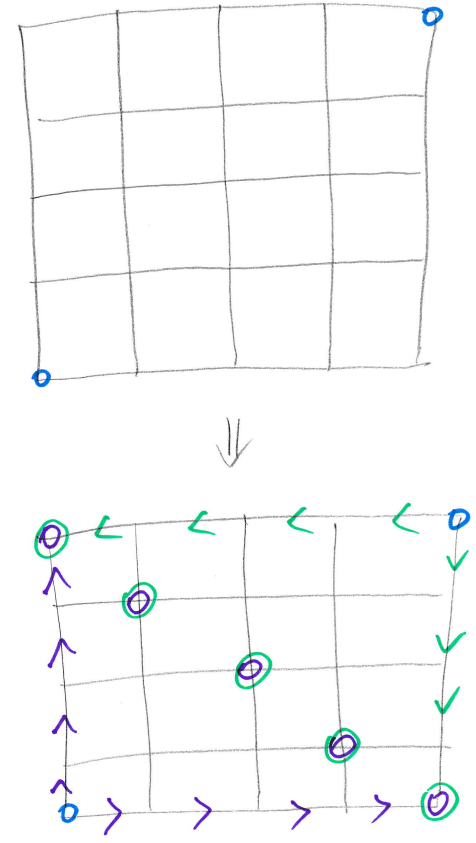
\includegraphics[width=0.7\linewidth]{voronoi1}
\caption{Calculate the Manhattan voronoi}
\label{voronoi1}
\end{figure}


\begin{figure}[h]
\centering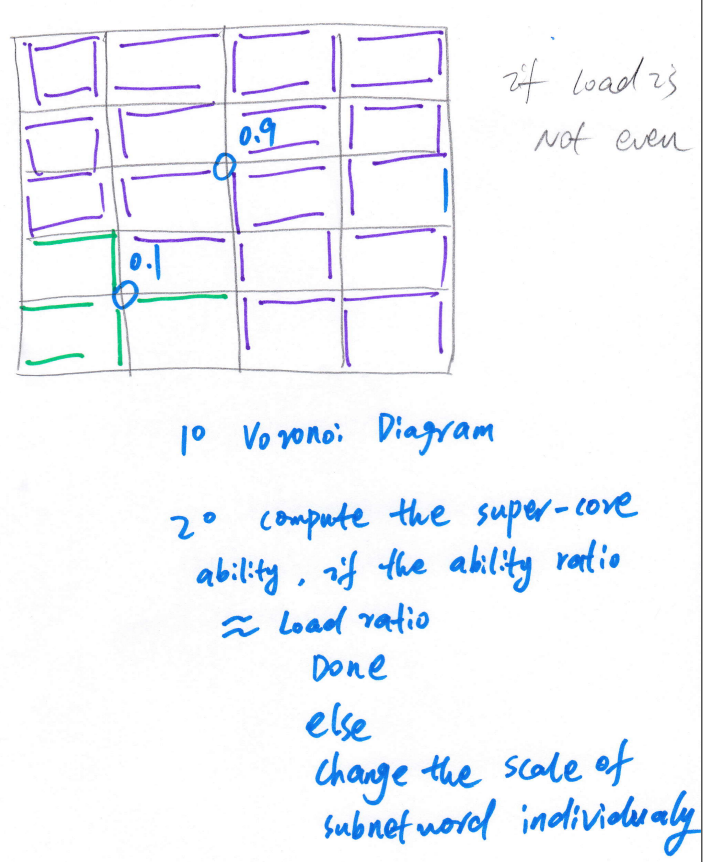
\includegraphics[width=0.7\linewidth]{voronoi2}
\caption{Load balance based on the load fraction}
\label{voronoi2}
\end{figure}

\section{Optimal Mass Transport}

\begin{itemize}
\item If we know the number of source
\item If we know the load fraction of each source
\item To decide the location of each base.
\end{itemize}

The main assumption is here. 

\begin{itemize}
\item All the unit core are the same.
\item The number of core is approximate with the ability with the power of corresponding subgraph.
\item The number of core is approximate with the area of each subgraph.
\end{itemize}

So the problem transfer a work load fraction to a problem which is divide the whole graph to a target area(measure).

If the target workload are equal, we also can choose the Centroidal Voronoi tessellation.


\section{Experiment}

\begin{itemize}
\item PDE simulation
\item Superposition
\item Processor Equivalence simulation.
\end{itemize}

\section{Conclusion}


%% The Appendices part is started with the command \appendix;
%% appendix sections are then done as normal sections
%% \appendix

%% \section{}
%% \label{}

%% References
%%
%% Following citation commands can be used in the body text:
%% Usage of \cite is as follows:
%%   \cite{key}          ==>>  [#]
%%   \cite[chap. 2]{key} ==>>  [#, chap. 2]
%%   \citet{key}         ==>>  Author [#]

%% References with bibTeX database:

\bibliographystyle{model1-num-names}
\bibliography{sample.bib}

%% Authors are advised to submit their bibtex database files. They are
%% requested to list a bibtex style file in the manuscript if they do
%% not want to use model1-num-names.bst.

%% References without bibTeX database:

% \begin{thebibliography}{00}

%% \bibitem must have the following form:
%%   \bibitem{key}...
%%

% \bibitem{}

% \end{thebibliography}


\end{document}

%%
%% End of file `elsarticle-template-1-num.tex'.